\begin{textbox}{\href{https://compneuro.neuromatch.io/tutorials/W1D2_ModelFitting/chapter_title.html}{Linear regression with MSE }}
\begin{subbox}{subbox}{Mean Squared Error (MSE)}
\scriptsize
\textbf{Linear least squares regression} is an old but gold  optimization procedure that we are going to use for data fitting. Least squares (LS) optimization problems are those in which the objective function is a quadratic function of the
parameter(s) being optimized.

Suppose you have a set of measurements: for each data point or measurement, you have $y_{i}$ (the "dependent" variable) obtained for a different input value, $x_{i}$ (the "independent" variable).  Suppose we believe the measurements are proportional to the input values, but are corrupted by some (random) measurement errors, $\epsilon_{i}$, that is:
\begin{equation}
y_{i}= \theta x_{i}+\epsilon_{i}
\end{equation}
for some unknown slope parameter $\theta.$ The least squares regression problem uses \textbf{mean squared error (MSE)} as its objective function, it aims to find the value of the parameter $\theta$ by minimizing the average of squared errors:
\begin{equation}
\min _{\theta} \frac{1}{N}\sum_{i=1}^{N}\left(\epsilon_{i}\right)^{2}
\end{equation}
\begin{equation}
\min _{\theta} \frac{1}{N}\sum_{i=1}^{N}\left(y_{i}-\theta x_{i}\right)^{2}
\end{equation}
\centering
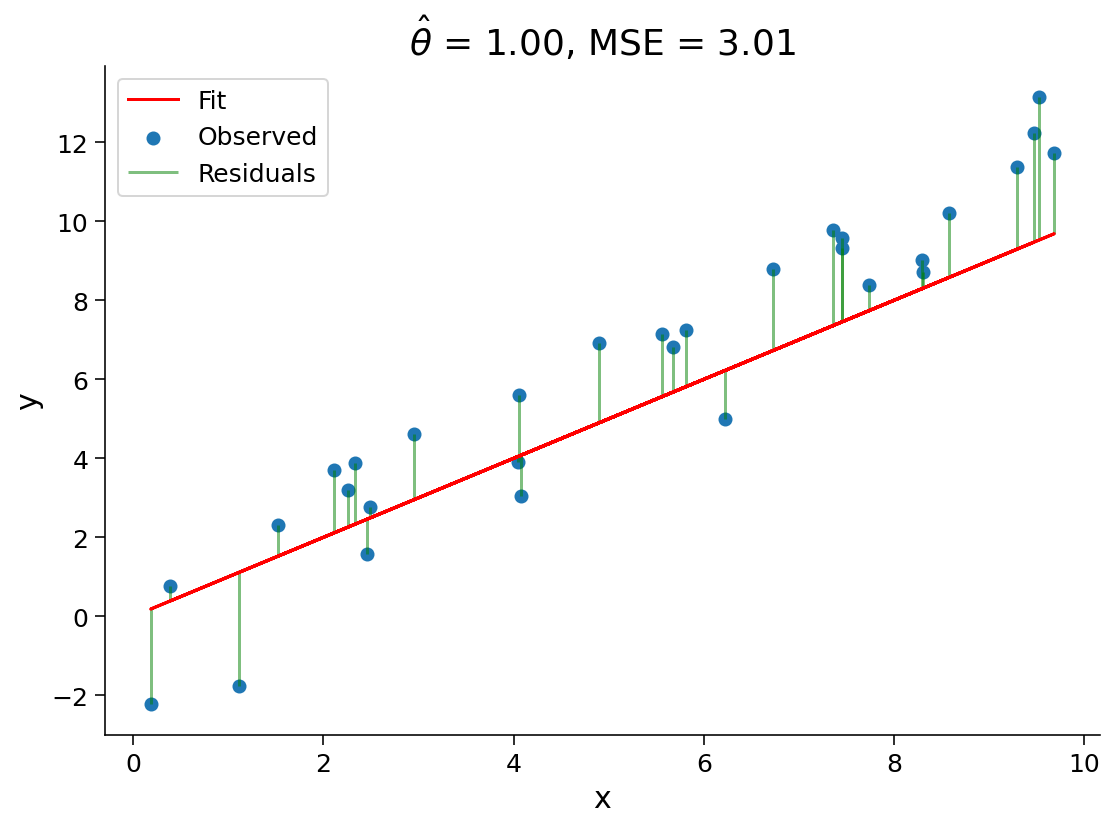
\includegraphics[scale=0.15]{Figures/ModelFitting/MFFigure1.png}
\end{subbox}
%%%%%%%%%%%%%%%%%%%%%%%%%%%%%%%%%%%%%%%%%%%%%%%%%%
\begin{subbox}{subbox}{Least-Squares Optimization}
\scriptsize
The MSE value relies on a grid of hand-specified values. If we didn't pick a good range to begin with, or with enough granularity, we might miss the best possible estimator. Instead of finding the minimum MSE from a set of candidate estimates, let's solve for it analytically.
We can do this by minimizing the cost function. Mean squared error is a convex objective function, therefore we can compute its minimum using calculus for find the best estimate: \begin{align}
\hat\theta = \frac{\mathbf{x}^\top \mathbf{y}}{\mathbf{x}^\top \mathbf{x}}
\end{align}

where $\mathbf{x}$ and $\mathbf{y}$ are vectors of data points.

\end{subbox}

\end{textbox}
%%%%%%%%%%%%%%%%%%%%%%%%% 
%%%%%%%%%%%%%%%%%%%%%%%%%
\begin{textbox}{\href{https://compneuro.neuromatch.io/tutorials/W1D2_ModelFitting/student/W1D2_Tutorial2.html}{Linear regression with MLE }  }
\begin{subbox}{subbox}{ Gaussian noise}
\scriptsize
In the MSE we made the assumption that the data was drawn from a linear relationship with noise added.

In that case we treated the noise as simply a nuisance, but what if we factored it directly into our model?

The noise component $\epsilon$ is often modeled as a random variable drawn from a Gaussian distribution (also called the normal distribution).

The Gaussian distribution is described by its probability density function (pdf)
\begin{align}
\mathcal{N}(x; \mu, \sigma^2) = \frac{1}{\sqrt{2\pi\sigma^2}}e^{-\frac{1}{2\sigma^2}(x-\mu)^2}
\end{align}

and is dependent on two parameters: the mean $\mu$ and the variance $\sigma^2$. We often consider the noise signal to be Gaussian "white noise", with zero mean and unit variance
$\epsilon \sim \mathcal{N}(0, 1).
$

\end{subbox}
%%%%%%%%%%%%%%%%%%%%%%%%%%%%%%%%%%%%%%%%%%%%%%%%%%
\begin{subbox}{subbox}{Probabilistic Models}
\scriptsize
Consider again our simplified model $y = \theta x + \epsilon$ where the noise has zero mean and unit variance $\epsilon \sim \mathcal{N}(0, 1)$. We can now also treat $y$ as a random variable drawn from a Gaussian distribution where $\mu = \theta x$ and $\sigma^2 = 1$, 
$y \sim \mathcal{N}(\theta x, 1),
$

which is to say that the probability of observing $y$ given $x$ and parameter $\theta$ is
\begin{align}
p(y|x,\theta) = \frac{1}{\sqrt{2\pi}}e^{-\frac{1}{2}(y-\theta x)^2}
\end{align}

\end{subbox}

\begin{subbox}{subbox}{Likelihood Estimation}
\scriptsize
 Given the inherent uncertainty when dealing in probabilities, we talk about the likelihood that some estimate $\hat{\theta}$ fits our data. The likelihood function $\mathcal{L}(\theta)$ is equal to the probability density function parameterized by that $\theta$:
\begin{align}
\mathcal{L}(\theta|x,y) = p(y|x,\theta) = \frac{1}{\sqrt{2\pi\sigma^2}}e^{-\frac{1}{2\sigma^2}(y-\theta x)^2}
\end{align}
Since we have assumed that the noise affects each output independently, we can factorize the likelihood, and write:
\begin{align}
\mathcal{L}(\theta|\mathbf{x}, \mathbf{y}) = \prod_{i=1}^N \mathcal{L}(\theta|x_i,y_i),
\end{align}
where we have $N$ data points $\mathbf{x} = [x_1,...,x_N]$ and $\mathbf{y} = [y_1,...,y_N]$.
\end{subbox}
\end{textbox}
%%%%%%%%%%%%%%%%%%%%%%%%% 
%%%%%%%%%%%%%%%%%%%%%%%%%
\begin{textbox}{\href{https://compneuro.neuromatch.io/tutorials/W1D2_ModelFitting/student/W1D2_Tutorial2.html}{Linear regression with MLE }   }
\begin{subbox}{subbox}{Finding the Maximum Likelihood Estimator (MLE)}
\scriptsize
We want to find the parameter value $\hat\theta$ that makes our data set most likely:

\begin{align}
\hat{\theta}_{\textrm{MLE}} = \underset{\theta}{\operatorname{argmax}} \mathcal{L}(\theta|X,Y) 
\end{align}

We discussed how taking the logarithm of the likelihood helps with numerical stability, the good thing is that it does so without changing the parameter value that maximizes the likelihood. Indeed, the $\log()$ function is *monotonically increasing*, which means that it preserves the order of its inputs. So we have:

\begin{align}
\hat{\theta}_{\textrm{MLE}} = \underset{\theta}{\operatorname{argmax}} \sum_{i=1}^m \textrm{log} \mathcal{L}(\theta|x_i,y_i) 
\end{align}

Now substituting our specific likelihood function and taking its logarithm, we get:
\begin{align}
\hat{\theta}_{\textrm{MLE}} = \underset{\theta}{\operatorname{argmax}} [-\frac{N}{2} \operatorname{log} 2\pi\sigma^2 - \frac{1}{2\sigma^2}\sum_{i=1}^N (y_i-\theta x_i)^2].
\end{align}

Note that maximizing the log likelihood is the same as minimizing the negative log likelihood (in practice optimization routines are developed to solve minimization not maximization problems). Because of the convexity of this objective function, we can take the derivative of our negative log likelihhood, set it to 0, and solve - just like our solution to minimizing MSE.

\begin{align}
\frac{\partial\operatorname{log}\mathcal{L}(\theta|x,y)}{\partial\theta}=\frac{1}{\sigma^2}\sum_{i=1}^N(y_i-\theta x_i)x_i = 0
\end{align}
\centering
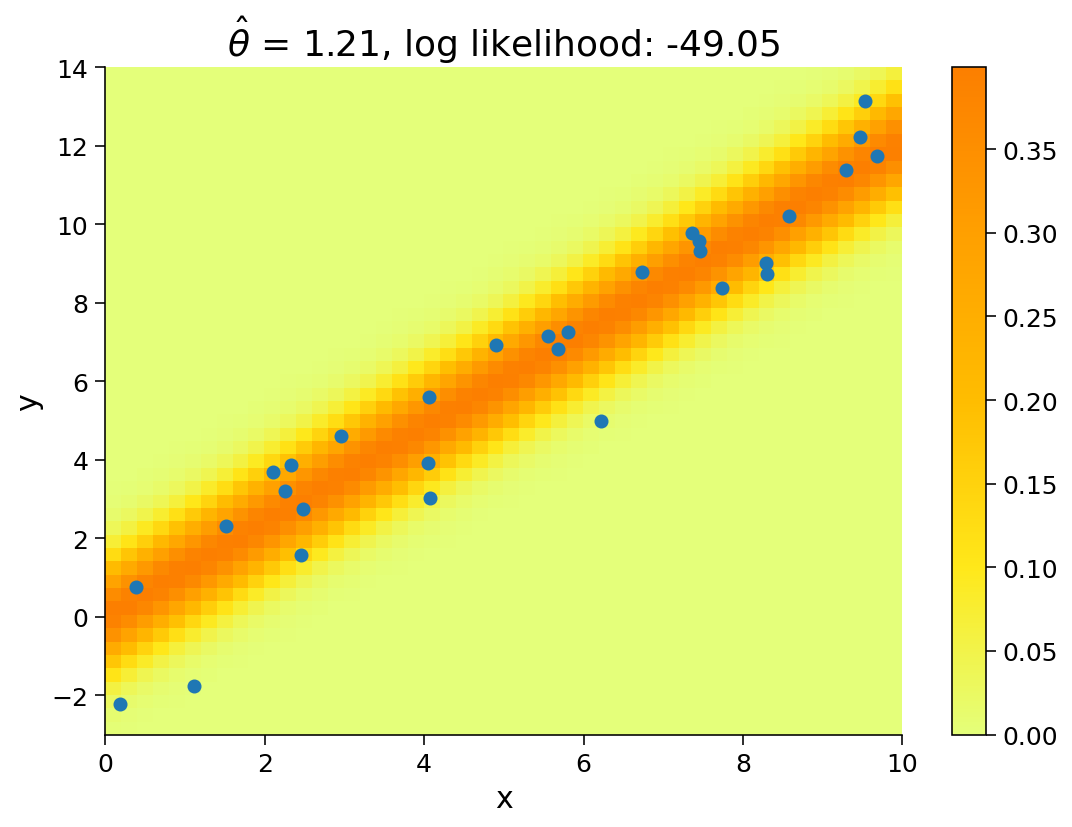
\includegraphics[scale=0.2]{Figures/ModelFitting/MFFigure2.png}
\end{subbox}
\end{textbox}
%%%%%%%%%%%%%%%%%%%%%%%%% 
%%%%%%%%%%%%%%%%%%%%%%%%%
\begin{textbox}{\href{https://compneuro.neuromatch.io/tutorials/W1D2_ModelFitting/student/W1D2_Tutorial2.html}{Model Fitting} -  Confidence Intervals and Bootstrapping and Cross-validation}
\begin{subbox}{subbox}{\href{https://compneuro.neuromatch.io/tutorials/W1D2_ModelFitting/student/W1D2_Tutorial3.html}{Confidence Intervals and Bootstrapping }  }

\scriptsize

 Bootstrapping is a resampling procedure that allows to build confidence intervals around inferred parameter values.
It is a widely applicable and very practical method that relies on computational power and pseudo-random number generators (as opposed to more classical approaches than depend on analytical derivations)

The idea is to generate many new synthetic datasets from the initial true dataset by randomly sampling from it, then finding estimators for each one of these new datasets, and finally looking at the distribution of all these estimators to quantify our confidence.

Note that each new resampled datasets will be the same size as our original one, with the new data points sampled with replacement i.e. we can repeat the same data point multiple times. 

\centering
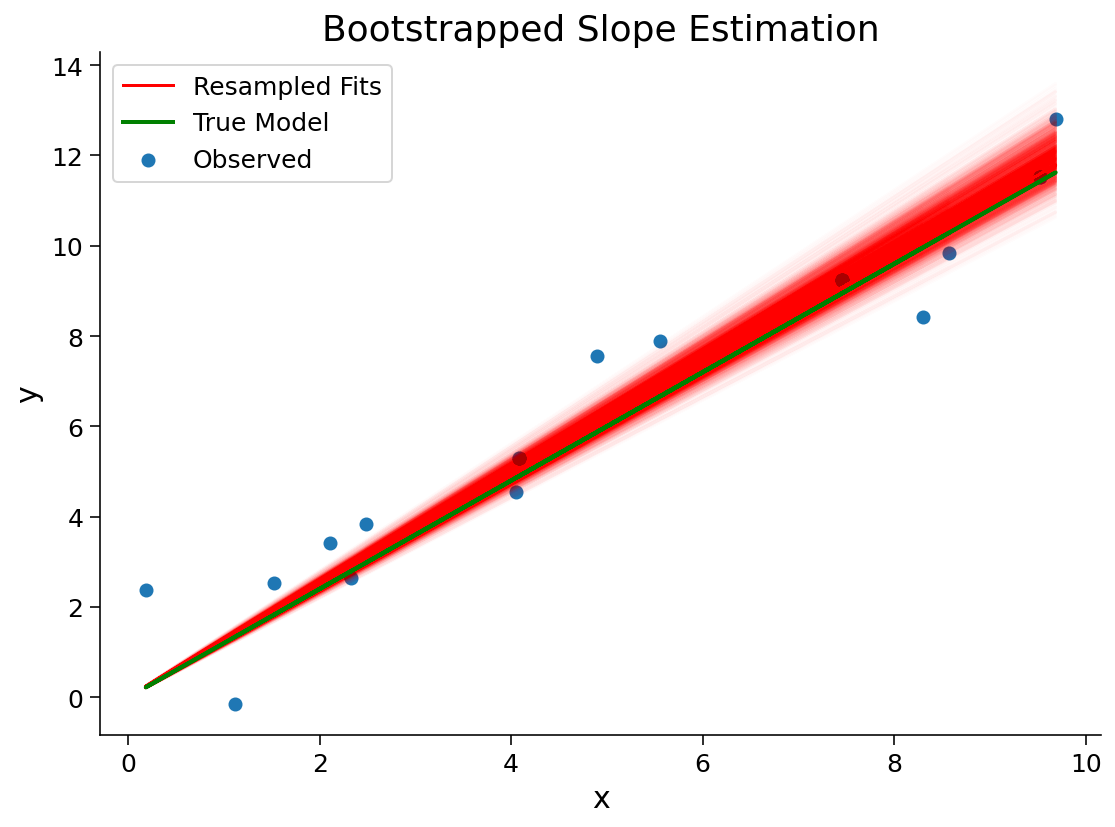
\includegraphics[scale=0.2]{Figures/ModelFitting/MFFigure3.png}

\end{subbox}
\begin{subbox}{subbox}{\href{https://compneuro.neuromatch.io/tutorials/W1D2_ModelFitting/student/W1D2_Tutorial6.html}{Cross-validation }  }

\scriptsize

A commonly used method for model selection is to ask how well the model predicts new data that it hasn't seen yet. But we don't want to use test data to do this, otherwise that would mean using it during the training process! One approach is to use another kind of held-out data which we call \textbf{validation data}: we do not fit the model with this data but we use it to select our best model.

We often have a limited amount of data though (especially in neuroscience), so we do not want to further reduce our potential training data by reassigning some as validation. Luckily, we can use \textbf{k-fold cross-validation}! In k-fold cross validation, we divide up the training data into k subsets (that are called \textit{folds}, see diagram below), train our model on the first k-1 folds, and then compute error on the last held-out fold.

\centering
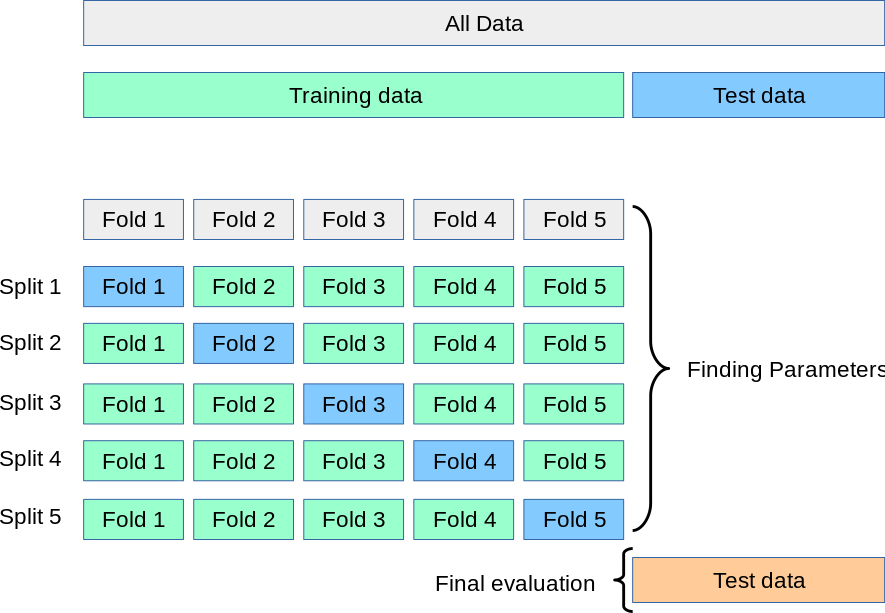
\includegraphics[scale=0.14]{Figures/ModelFitting/MFFigure7.png}

\end{subbox}
\end{textbox}
%%%%%%%%%%%%%%%%%%%%%%%%% 
%%%%%%%%%%%%%%%%%%%%%%%%%
%%%%%%%%%%%%%%%%%%%%%%%%% 
%%%%%%%%%%%%%%%%%%%%%%%%%
\begin{textbox}{\href{https://compneuro.neuromatch.io/tutorials/W1D2_ModelFitting/student/W1D2_Tutorial4.html}{Multiple Linear Regression and Polynomial Regression }   }
\begin{subbox}{subbox}{Multiple Linear Regression}
\scriptsize

We can easily extend univariate regression to the multivariate scenario by adding another parameter for each additional feature
\begin{align}
y = \theta_0 + \theta_1 x_1 + \theta_2 x_2 + ... +\theta_d x_d + \epsilon
\end{align}
where $\theta_0$ is the intercept and $d$ is the number of features (it is also the dimensionality of our input).

We can condense this succinctly using vector notation for a single data point
\begin{align}
y_i = \boldsymbol{\theta}^{\top}\mathbf{x}_i + \epsilon
\end{align}

and fully in matrix form

\begin{align}
\mathbf{y} = \mathbf{X}\boldsymbol{\theta} + \mathbf{\epsilon}
\end{align}

where $\mathbf{y}$ is a vector of measurements, $\mathbf{X}$ is a matrix containing the feature values (columns) for each input sample (rows), and $\boldsymbol{\theta}$ is our parameter vector.
This matrix $\mathbf{X}$ is often referred to as the design matrix.
To find an optimal vector of parameters $\boldsymbol{\hat\theta}$ we use:
\begin{align}
\boldsymbol{\hat\theta} = (\mathbf{X}^\top\mathbf{X})^{-1}\mathbf{X}^\top\mathbf{y}.
\end{align}
\end{subbox}
\begin{subbox}{subbox}{Polynomial Regression}
\scriptsize
The polynomial regression is an extension of linear regression, the dependent variable $y$ given the input values $x$. The key change is the type of relationship between inputs and outputs that the model can capture.
With polynomial regression, we model the outputs as a polynomial equation based on the inputs. For example, we can model the outputs as:

\begin{align}
y & = \theta_0 + \theta_1 x + \theta_2 x^2 + \theta_3 x^3 + \epsilon
\end{align}
We can change how complex a polynomial is fit by changing the order of the polynomial. The order of a polynomial refers to the highest power in the polynomial. 

\centering
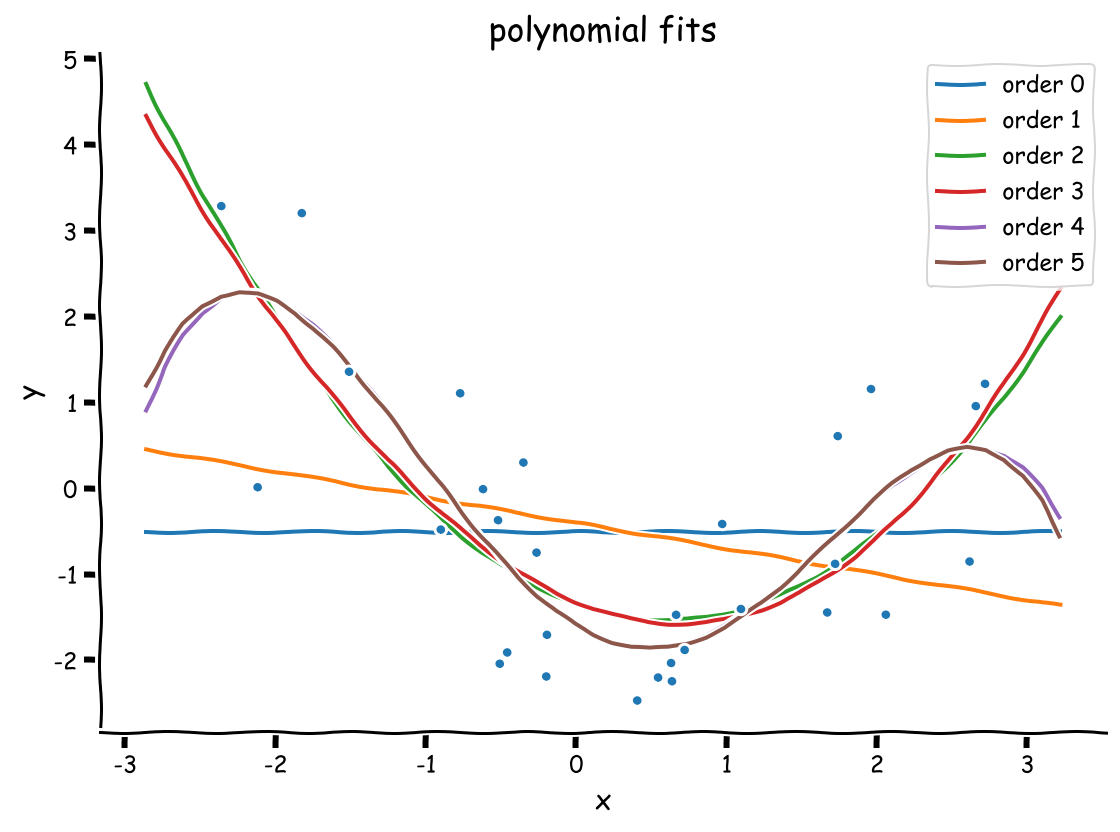
\includegraphics[scale=0.1]{Figures/ModelFitting/MFFigure4.png}
\end{subbox}
\end{textbox}
%%%%%%%%%%%%%%%%%%%%%%%%% 
%%%%%%%%%%%%%%%%%%%%%%%%%
\begin{textbox}{\href{https://compneuro.neuromatch.io/tutorials/W1D2_ModelFitting/student/W1D2_Tutorial5.html}{Model Selection: Bias-variance trade-off }  }
\begin{subbox}{subbox}{Train and Test}
\scriptsize

 The data used for the fitting procedure for a given model is the \textbf{training data}. We computed MSE on the training data of our polynomial regression models and compared training MSE across models. An additional important type of data is \textbf{test data}. This is held-out data that is not used (in any way) during the fitting procedure. When fitting models, we often want to consider both the train error (the quality of prediction on the training data) and the test error (the quality of prediction on the test data).
 
\centering
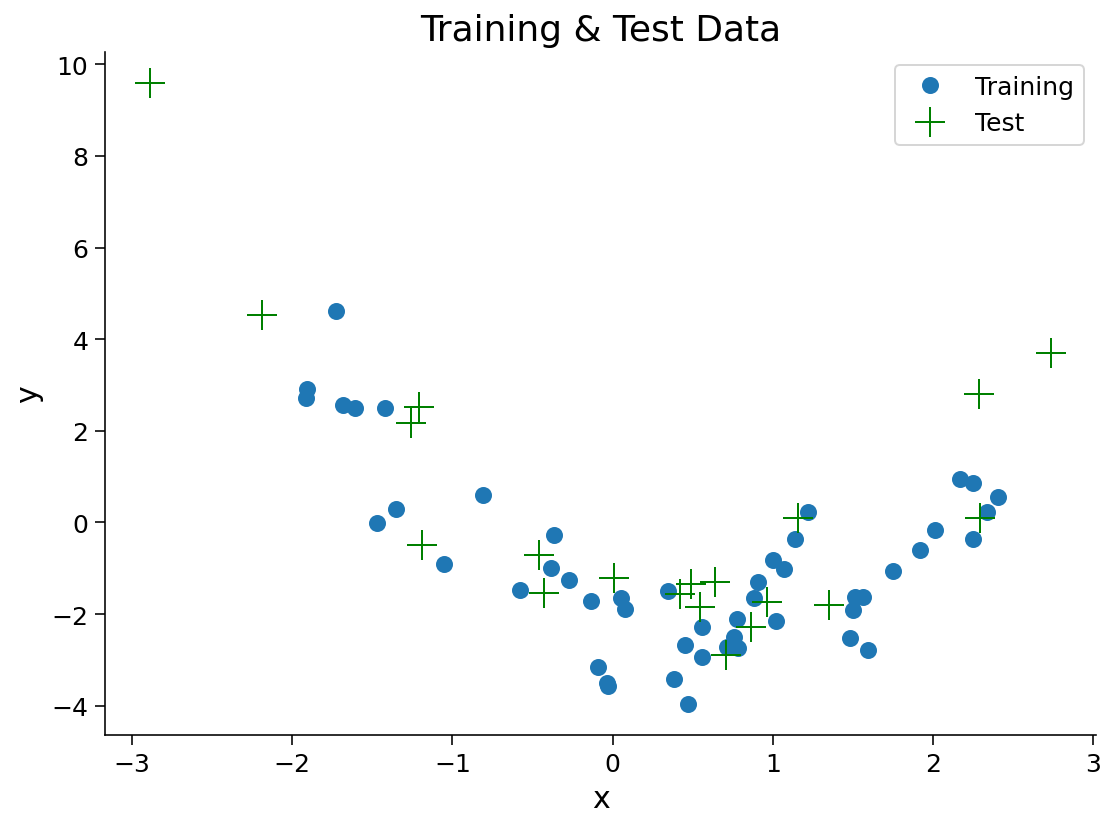
\includegraphics[scale=0.2]{Figures/ModelFitting/MFFigure5.png}
\end{subbox}
\begin{subbox}{subbox}{Bias-Variance Tradeoff}
\scriptsize
Finding a good model can be difficult. One of the most important concepts to keep in mind when modeling is the \textbf{bias-variance tradeoff}. 

\textbf{Bias} is the difference between the prediction of the model and the corresponding true output variables you are trying to predict. Models with high bias will not fit the training data well since the predictions are quite different from the true data. These high bias models are overly simplified - they do not have enough parameters and complexity to accurately capture the patterns in the data and are thus \textbf{underfitting}.


\textbf{Variance} refers to the variability of model predictions for a given input. Essentially, do the model predictions change a lot with changes in the exact training data used? Models with high variance are highly dependent on the exact training data used - they will not generalize well to test data. These high variance models are \textbf{overfitting} to the data.

\centering
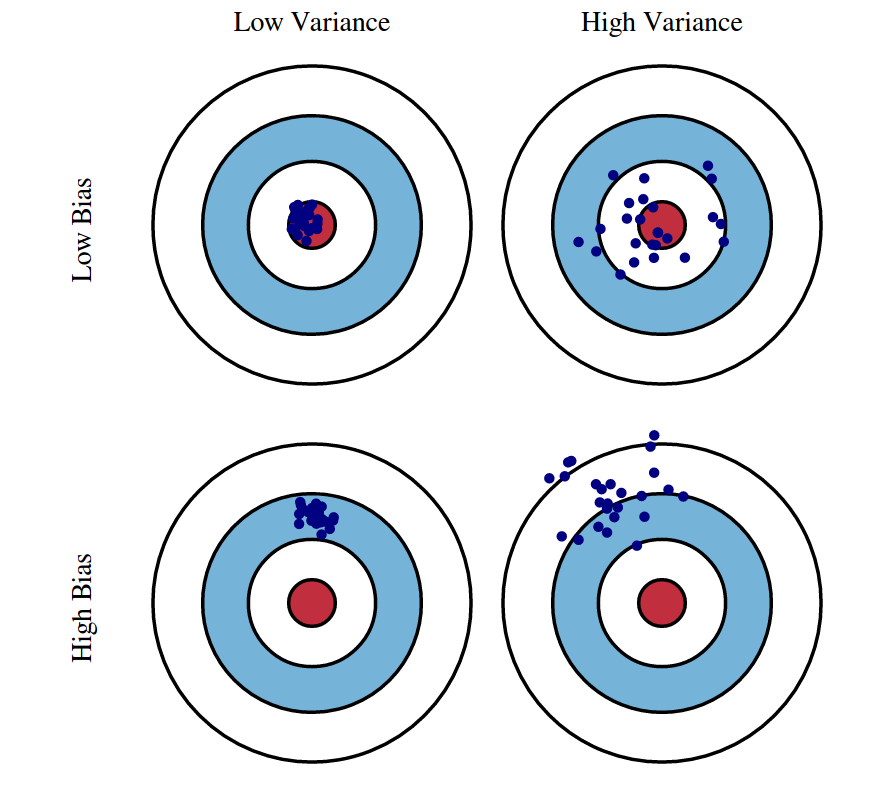
\includegraphics[scale=0.13]{Figures/ModelFitting/MFFigure6.png}
\end{subbox}
\end{textbox}